% 非互換なパッケージに自動でパッチを当てる
% https://qiita.com/wtsnjp/items/76557b1598445a1fc9da
\RequirePackage{plautopatch}
% pdfpagesの依存パッケージのエラー回避
% https://okumuralab.org/tex/mod/forum/discuss.php?d=2956
% https://github.com/aminophen/gentombow/issues/9
\plautopatchdisable{eso-pic}
% documentclassでdvipdfmx指定をするので個別パッケージでのドライバ指定は不要
% https://qiita.com/Aruneko/items/13e015bce0112143f277
\documentclass[autodetect-engine, dvi=dvipdfmx, 10pt, a4paper, ja=standard]{bxjsarticle}

% 印刷時の用紙サイズ設定
\usepackage{bxpapersize}% これでOK!

% pdf-version
\usepackage[1.4]{bxpdfver}

% 日本語環境での字体修正
\usepackage{otf}
% フォントエンコーディングの名前をオプションで指定する
\usepackage[T1]{fontenc}
\usepackage{lmodern}% Latin Modern フォントを使う

% graphicx
\usepackage{graphicx}
\usepackage{grffile}% include graphicsの画像ファイル名の制限を撤廃

% \begin{comment} ... \end{comment} で複数行コメントアウト
\usepackage{comment}

% 数学系 インライン数式を \[ \] と書く癖をつける
\usepackage{amsmath,amssymb,amsthm}
\usepackage{amsfonts}
\usepackage{mathtools}
\usepackage{bm} % bold math

% 化学
\usepackage[version=4]{mhchem}

% SI単位系
\usepackage{siunitx}

% 表関連
\usepackage{multirow} % 表のセルの結合
\usepackage{booktabs} % 表の線がすごくなる. Table Generatorを使うときはbooktabsモードにする
\usepackage{caption} % キャプションをいじる
\usepackage{float} % 図表を絶対にそこに置く確固たる意思

% その他便利な子
\usepackage{pdfpages} % pdfを挿入
\usepackage[hyphens]{url} % urlをきれいに表示する
\usepackage{ulem} % 下線を強化
\usepackage[at]{easylist} % @をつかって箇条書き
% \usepackage{minted}
% \usepackage{termsim} % ターミナルを再現...誰得?

% ハイパーリンクを生成
% sectionなどで数式を使う場合は \texorpdfstring{texstring}{pdfstring}をする
\usepackage{hyperref}
\usepackage{pxjahyper}
\usepackage{footnotebackref} % 脚注から本文へ飛べる


% ここからはソースコードを表示する設定
\usepackage{listings, plistings, color}
\renewcommand{\lstlistingname}{Code}
\definecolor{OliveGreen}{rgb}{0.0,0.6,0.0}
\definecolor{Orenge}{rgb}{0.89,0.55,0}
\definecolor{SkyBlue}{rgb}{0.28, 0.28, 0.95}
\lstset{
    language={Ruby}, % 言語の指定
    basicstyle={\ttfamily},
    identifierstyle={\small},
    commentstyle={\smallitshape},
    keywordstyle={\small\bfseries},
    ndkeywordstyle={\small},
    stringstyle={\small\ttfamily},
    frame={tb},
    breaklines=true,
    columns=[l]{fullflexible},
    numbers=left,
    xrightmargin=0zw,
    xleftmargin=3zw,
    numberstyle={\scriptsize},
    stepnumber=1,
    numbersep=1zw,
    lineskip=-0.5ex,
    stepnumber=1,       % 行数の増間
    numbersep=1zw,      % 行数の余白
    xrightmargin=0zw,   % 左の余白
    xleftmargin=2zw,    % 右の余白
    framexleftmargin=18pt,  % フレームからの左の余白
    keepspaces=true,    % スペースを省略せず保持
    lineskip=-0.2ex,    % 枠線の途切れ防止
    tabsize = 4,        % タブ数
    showstringspaces=false,  %文字列中の半角スペースを表示させない
    keywordstyle={\color{SkyBlue}},     %キーワード(int, ifなど)の書体指定
    commentstyle={\color{OliveGreen}},  %注釈の書体
    stringstyle=\color{Orenge}          %文字列
}

% \refだけで「図」や「式」を自動挿入
% https://zenn.dev/arks/articles/3697b25d03f8a8
% subfigureが文書にあると小節を参照する際に使う\subrefがおかしくなるので注意
%% increase link area for cross-references and autoname them, [130514]
\AtBeginDocument{\renewcommand{\ref}[1]{\mbox{\autoref{#1}}}}

\def\equationautorefname~#1\null{式(#1)\null}
\def\figureautorefname~#1\null{図#1\null}
\def\subfigureautorefname#1\null{図#1\null}
\def\tableautorefname~#1{表#1}
\def\lstlistingautorefname~#1{コード#1}

\def\partautorefname#1\null{第#1部\null}
\def\chapterautorefname#1\null{第#1章\null}
\def\sectionautorefname#1\null{#1節}
\def\subsectionautorefname~#1\null{#1節}
\def\subsubsectionautorefname#1\null{#1節}
\def\paragraphautorefname#1\null{#1段落}
\def\subparagraphautorefname#1\null{#1段落}

\def\Itemautorefname#1\null{項目#1\null}
\def\Hfootnoteautorefname#1\null{脚注#1\null}
\def\theoremautorefname#1\null{定理#1\null}
\def\FancyVerbLineautorefname#1\null{#1行\null}
% \def\pageautorefname#1\null{ページ#1\null}
\def\appendixautorefname#1\null{付録#1\null}


\title{MICS実験第一 J1課題レポート}
\author{学籍番号 2210342, 鈴木謙太郎}
\date{\today}
\begin{document}
\maketitle


% \bibliography{hoge} %hoge.bibから拡張子を外した名前
% \bibliographystyle{junsrt} %参考文献出力スタイル
% 使用する際は latex-workshop.latex.recipe.default を
% ptex2pdf (uplatex) → bibtex → ptex2pdf (uplatex) × 2
% に変更

\section{問題1}

\subsection{目的}

本問題では,FPGAにおいて入出力を接続する方法について理解することを目指す.


\subsection{原理・理論}

本問に限らずこの実験において用いるFPGAとは,Field Programmable Gate Arrayの略であり,
プログラムによって自由に書き換えられる論理素子である.

本実験では「Quartus」と呼ばれるソフトウェアを用いてGUI上で回路を設計し,
その回路をFPGAに書き込むことで,実際にハードウェア上で回路を動作させることができる.

実際に回路を構成する際は,入力ピン(ボタンやスイッチ,クロック信号など)と出力ピン(LEDなど)の間に
組み合わせ回路などを配置し,それらを接続することで入力に対して出力を得ることができる.

\subsection{回路のアルゴリズム・設計}

本問では,実験資料で示されたように,FPGAボード上のトグルスイッチや押しボタンスイッチに対して
LEDを接続することで,入力が与えられた際にLEDが点灯するような回路を設計する.

\subsection{実際に設計した回路}

\ref{fig:ex1}のような回路を設計した.

単純に入力スイッチのピンと出力LEDのピンを接続することで,
スイッチの入力がLEDの出力に反映されるようになっている.


\begin{figure}[htbp]
	\centering
	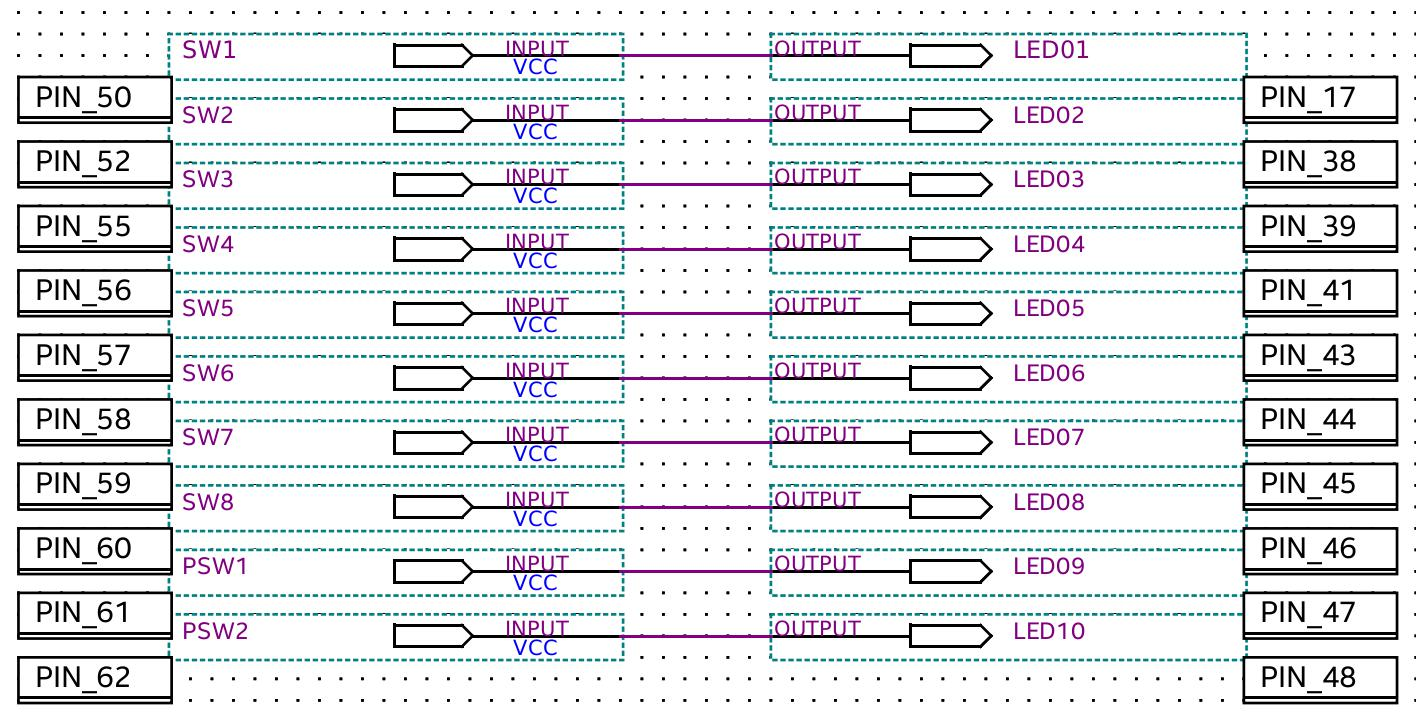
\includegraphics[width=0.8\textwidth]{asset/ex1-トリミング.jpg}
	\caption{問題1で設計した回路}
	\label{fig:ex1}
\end{figure}


\subsection{実験・測定結果}

実際にFPGAボードに書き込んだ結果,スイッチを操作することでLEDが点灯することが確認できた.

\ref{fig:ex1}からも分かる通り,この回路では各スイッチの入力は独立しているので,
同時に複数のスイッチを操作しても出力が変化することはなかった.

\section{問題2}

\subsection{目的}

本問では,ANDゲート,ORゲート,NOTゲートをはじめとするゲート回路を
FPGA上で動作させることを通じて,組み合わせ回路の設計方法を理解することを目指す.

\subsection{原理・理論}

組み合わせ回路とは,入力に対して出力が一意に定まる回路のことである.
この回路は,ゲート(AND,OR,NOTなど)のみを組み合わせることで構成される.


\subsection{回路のアルゴリズム・設計}
\label{sec:ex2-design}

本問では,2ビットの入力$x = x_1 x_0$と$y = y_1 y_0$に対して,
$x > y$のとき出力$z = 1$,それ以外のとき$z = 0$となる回路を設計する.
なお,これらの入力は符号なしの2進数として扱うものとする.

このような回路を作るにあたって,真理値表やカルノー図を用いることで
簡略化された効率のよい論理回路を作ることができる.

本問でも\ref{fig:ex2-karnaugh}のような真理値表とカルノー図を用いることで,
出力$z$の論理式を\ref{eq:ex2}のように求めた.

\begin{equation}
	\label{eq:ex2}
	z = x_0 y_1' y_0' + x_1 x_0 y_0' + x_1 y_1'
\end{equation}



\begin{figure}[htbp]
	\centering
	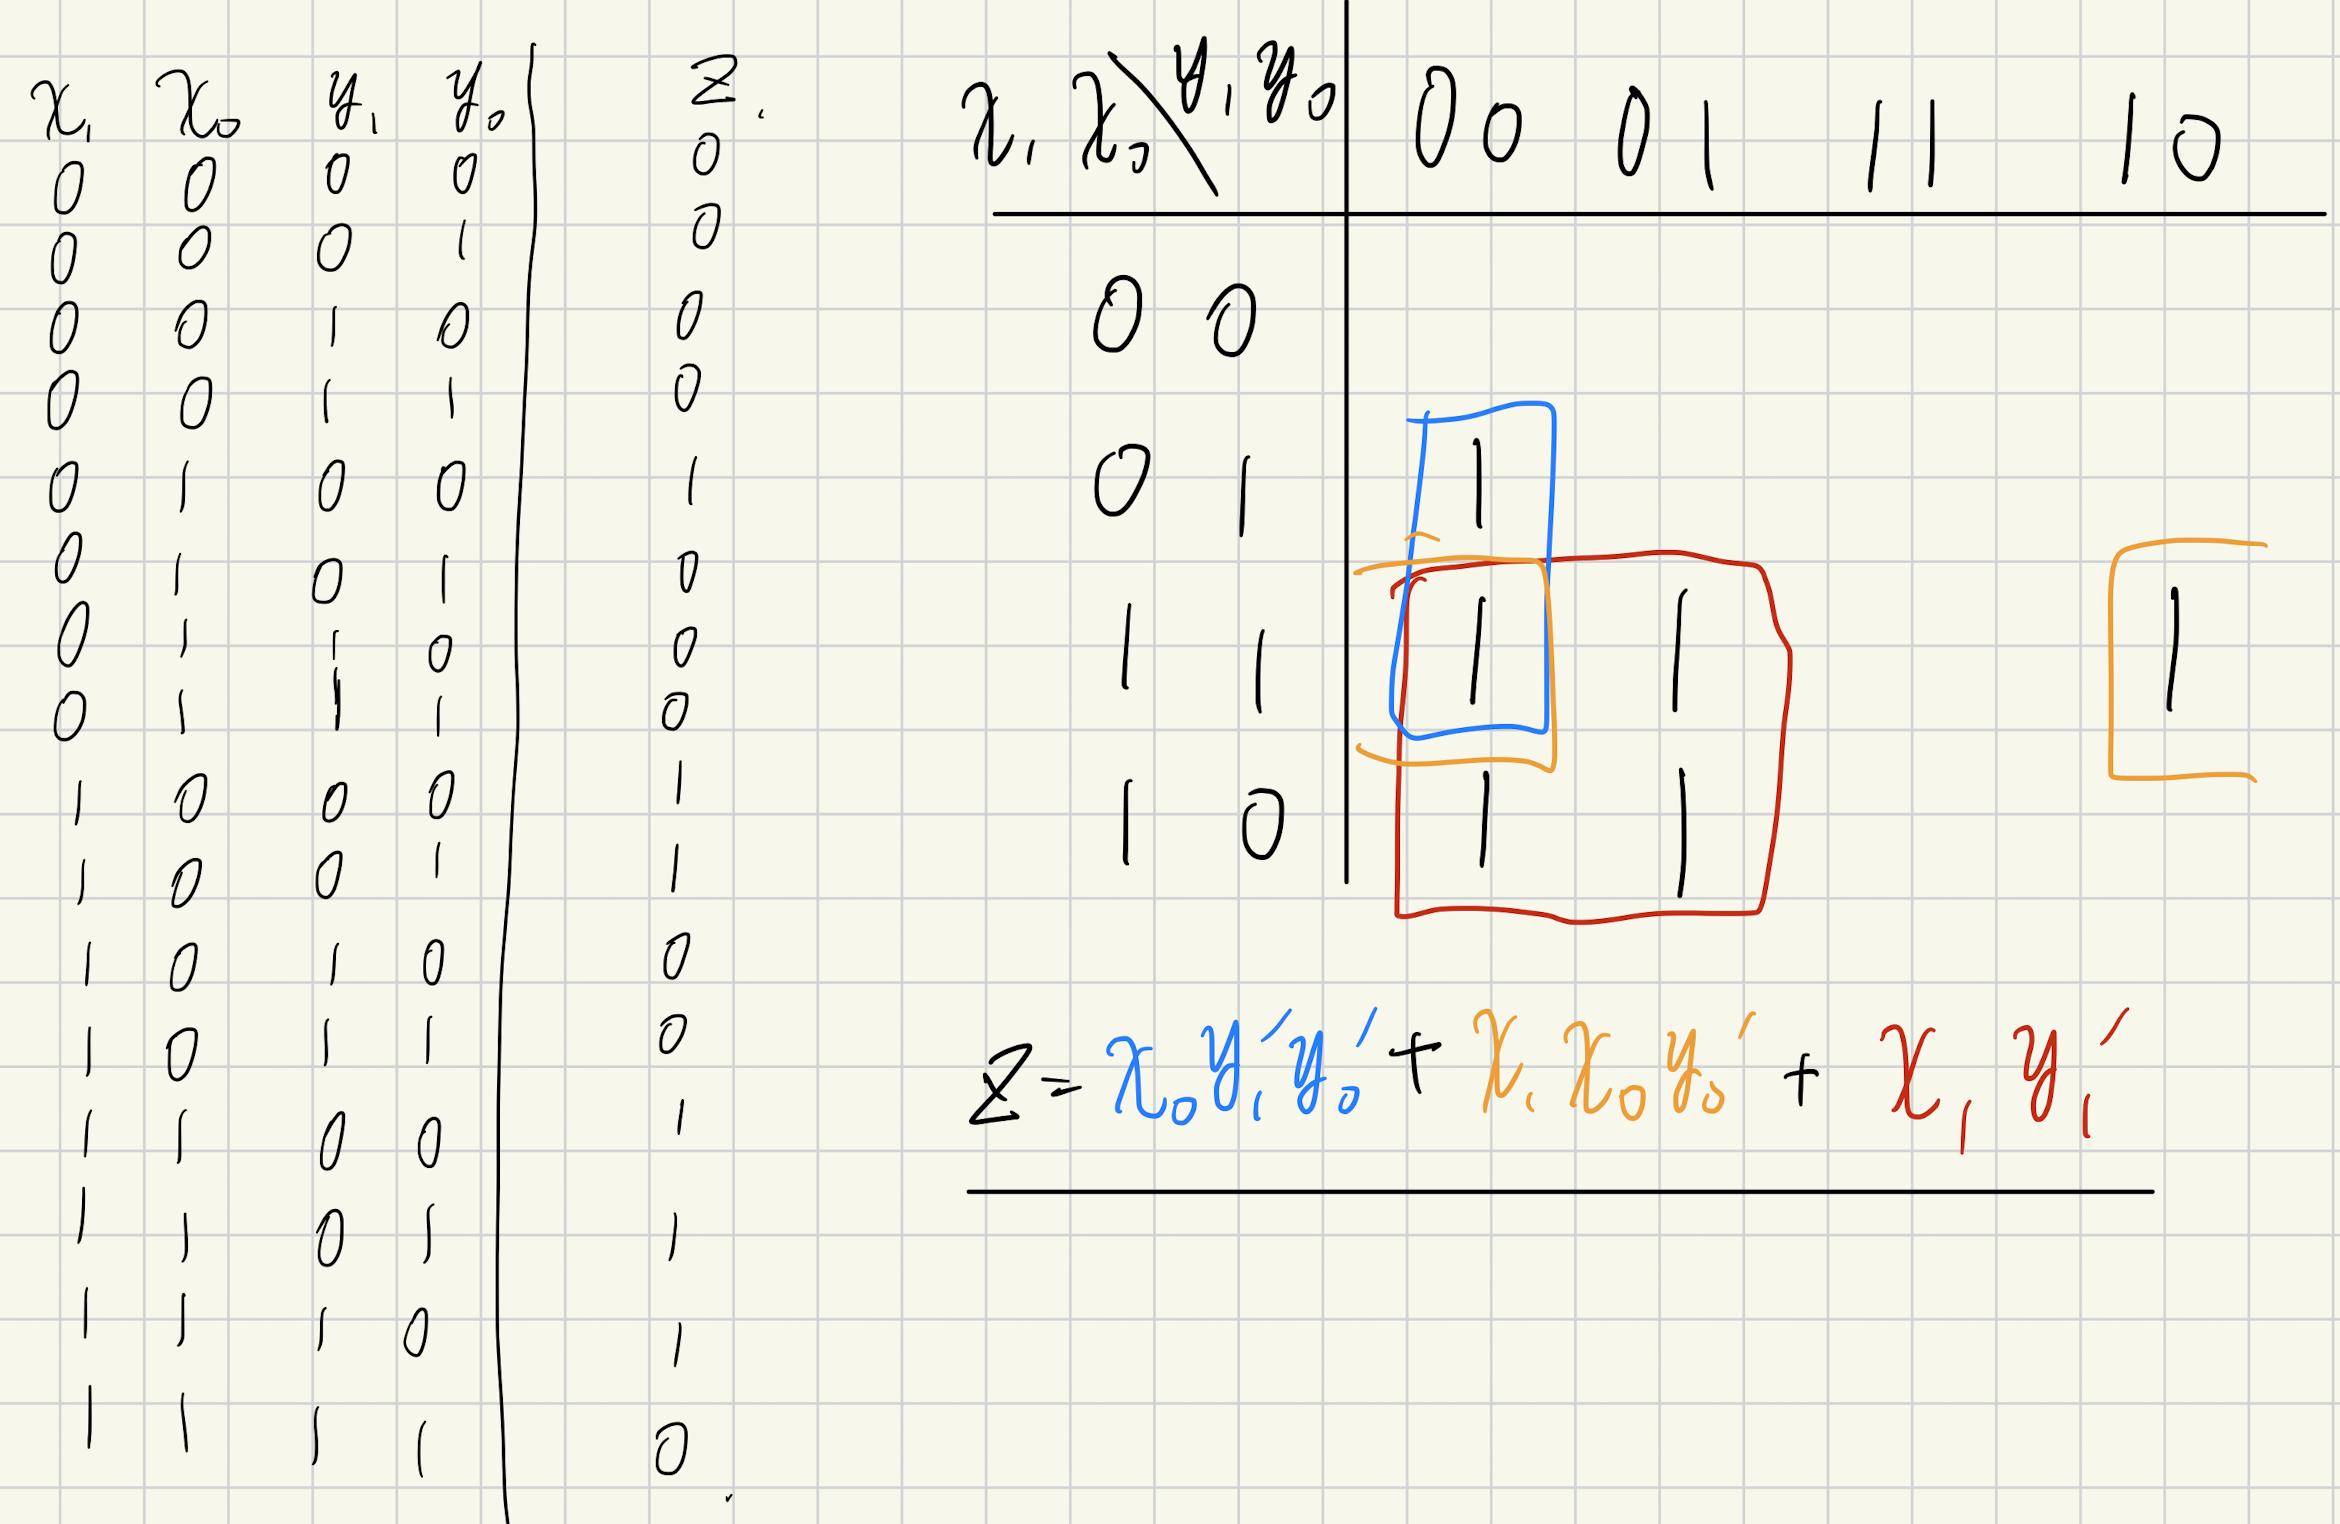
\includegraphics[width=0.8\textwidth]{asset/ex2_fig.png}
	\caption{問題2で用いた真理値表とカルノー図}
	\label{fig:ex2-karnaugh}
\end{figure}


実際の回路設計では,\ref{eq:ex2}の論理式をそのままゲートによる組み合わせ回路に変換することで,
期待する出力を得ることが可能である.
また,入力にはすべてトグルスイッチを用いた.

\subsection{実際に設計した回路}

\ref{eq:ex2}をもとに,\ref{fig:ex2}のような回路を設計した.

\begin{figure}[htbp]
	\centering
	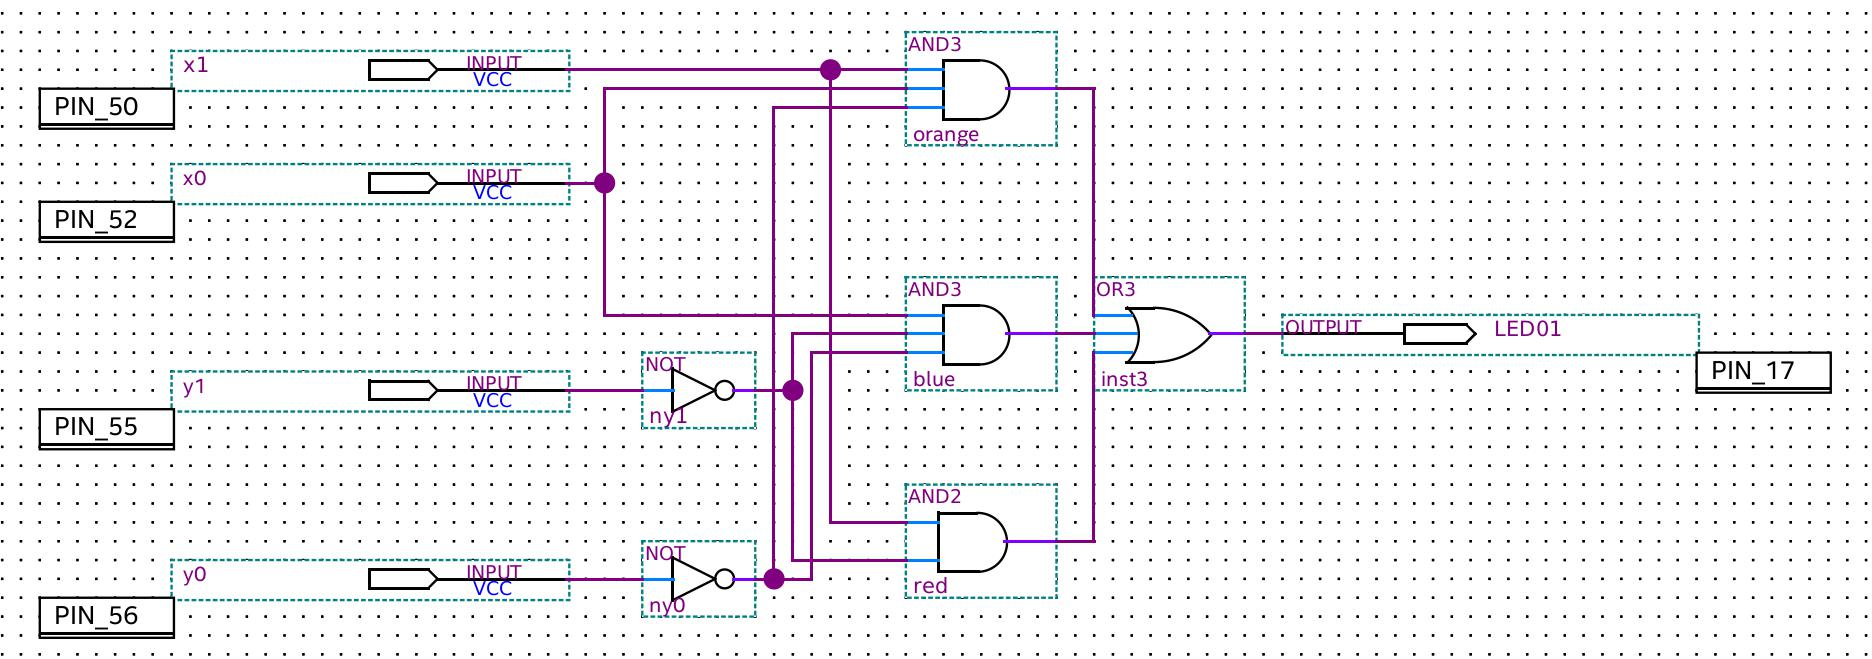
\includegraphics[width=0.8\textwidth]{asset/ex2_trim.jpg}
	\caption{問題2で設計した回路}
	\label{fig:ex2}
\end{figure}

\subsection{実験・測定結果}

実際にFPGAボードに書き込んだ結果,$x > y$のときに限りLEDが点灯し,$x = y$や$x < y$となるときは消灯することが確認できた.
よって,期待する出力を得ることができていると考えられる.

\section{問題3}

\subsection{目的}
本問では,D型フリップフロップを用いた微分回路を設計することで,順序回路の設計方法を理解することを目指す.

\subsection{原理・理論}
順序回路とは,組み合わせ回路とは異なり,出力が入力だけでなく過去の状態にも依存する回路のことである.
このような回路は,フリップフロップなどの記憶素子を用いることで設計することができる.

フリップフロップは,1ビットので0田を記憶できる素子である.特にD型フリップフロップは,
データとクロック信号を入力として受け取り,クロックが立ち上がるときにD入力の値を出力に反映する.
このような性質上,クロックはフリップフロップの動作を制御するために必要である.
この入力を人の手で正確に切り替えることは難しいため,FPGAボードに備え付けられたクロック信号発生器を用いる.

本問で作成する微分回路とは,入力信号の立ち上がりエッジを検出し,そのエッジが立ち上がるたびに出力信号をトグルする回路である.
このような回路を作成することで,人間がスイッチを1回押したときに,1クロックの長さのパルスを1回だけ出力することができる.
通常人がスイッチを操作すると,1クロック以上の信号が入力されてしまい,論理回路を正確にテストすることが難しいため,
微分回路は論理回路のテストにおいて非常に有用である.

\subsection{回路のアルゴリズム・設計}

本問では,クロック信号を入力として受け取り,その立ち上がりエッジを検出する微分回路を設計する.

フリップフロップなどを含む順序回路を設計する際には,出力が過去の状態に依存するため,
状態遷移図などを作成して設計を行うことが一般的である.

\ref{fig:ex3}のような回路を設計するにあたって,
便宜上左側のD型フリップフロップの入力を$D_0$, 出力を$Q_0$とし,
右側のD型フリップフロップの入力を$D_1$, 出力を$Q_1$とする.

\begin{figure}[htbp]
	\centering
	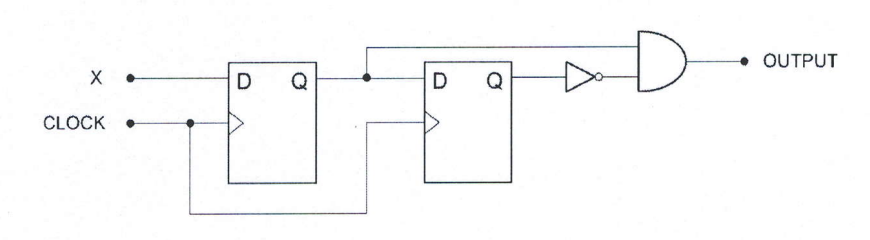
\includegraphics[width=0.8\textwidth]{asset/ex3_notebook.png}
	\caption{問題3で設計する微分回路の回路図(実験資料より引∑∑用)}
	\label{fig:ex3}
\end{figure}

この回路の真理値表は\ref{fig:ex3-tf}のようになった.

\begin{figure}[H]
	\centering
	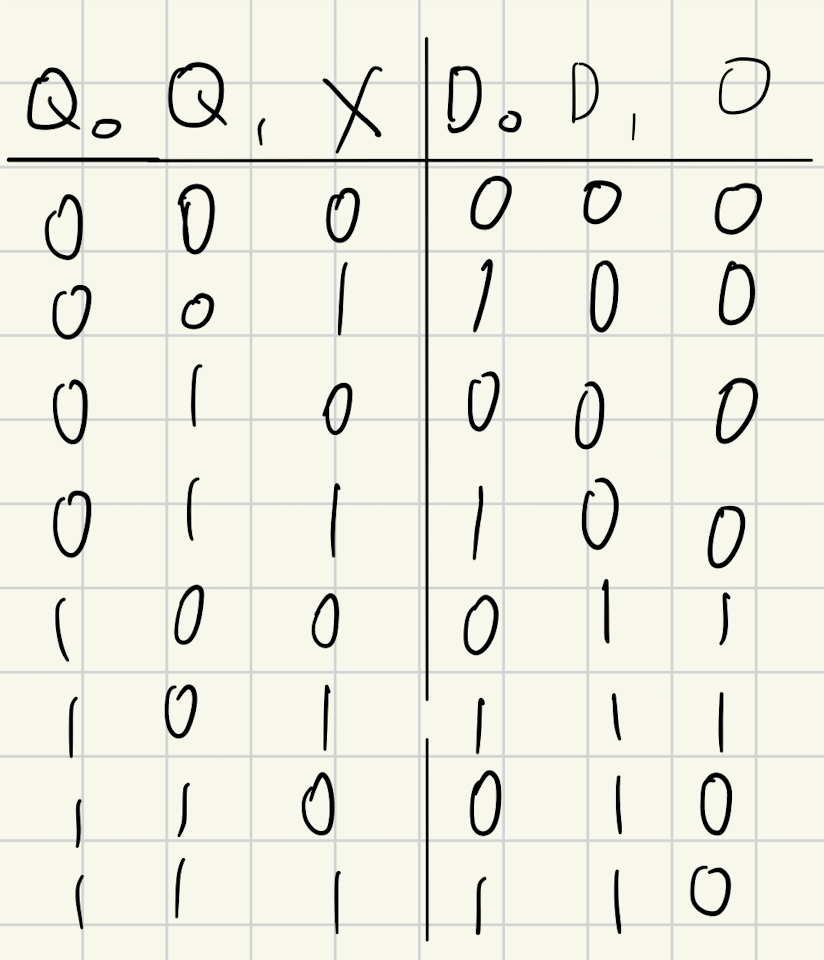
\includegraphics[width=0.8\textwidth]{asset/ex3_tf.png}
	\caption{問題3で用いた真理値表}
	\label{fig:ex3-tf}
\end{figure}

これの真理値表をもとに,\ref{fig:ex3-state}のような状態遷移図を作成した.

\begin{figure}[H]
	\centering
	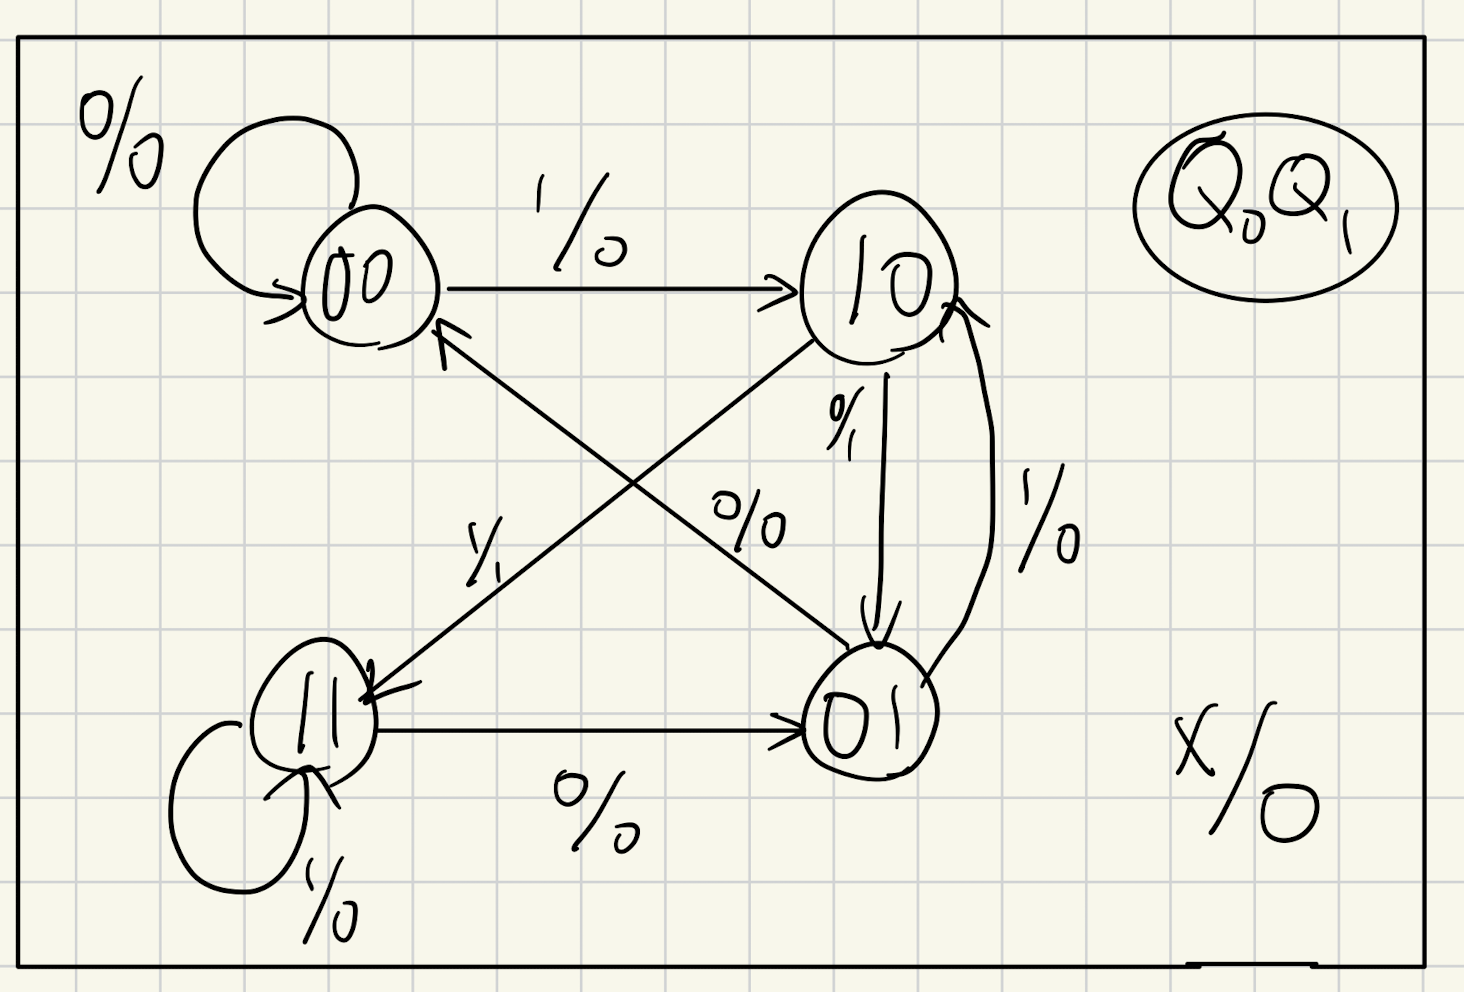
\includegraphics[width=0.8\textwidth]{asset/ex3_state.png}
	\caption{問題3で用いた状態遷移図}
	\label{fig:ex3-state}
\end{figure}

ここで,状態00と状態01に注目すると,ともに0を入力すると0を出力して状態00に遷移し,
1を入力すると1を出力して状態10に遷移することが分かる.よって,この2つの状態は同じものとみなせる.

このような同じ状態が複数ある場合,その状態への遷移とその状態からの遷移をまとめることで,
状態遷移図を\ref{fig:ex3-state-refine}のように簡略化することができる.

\begin{figure}[H]
	\centering
	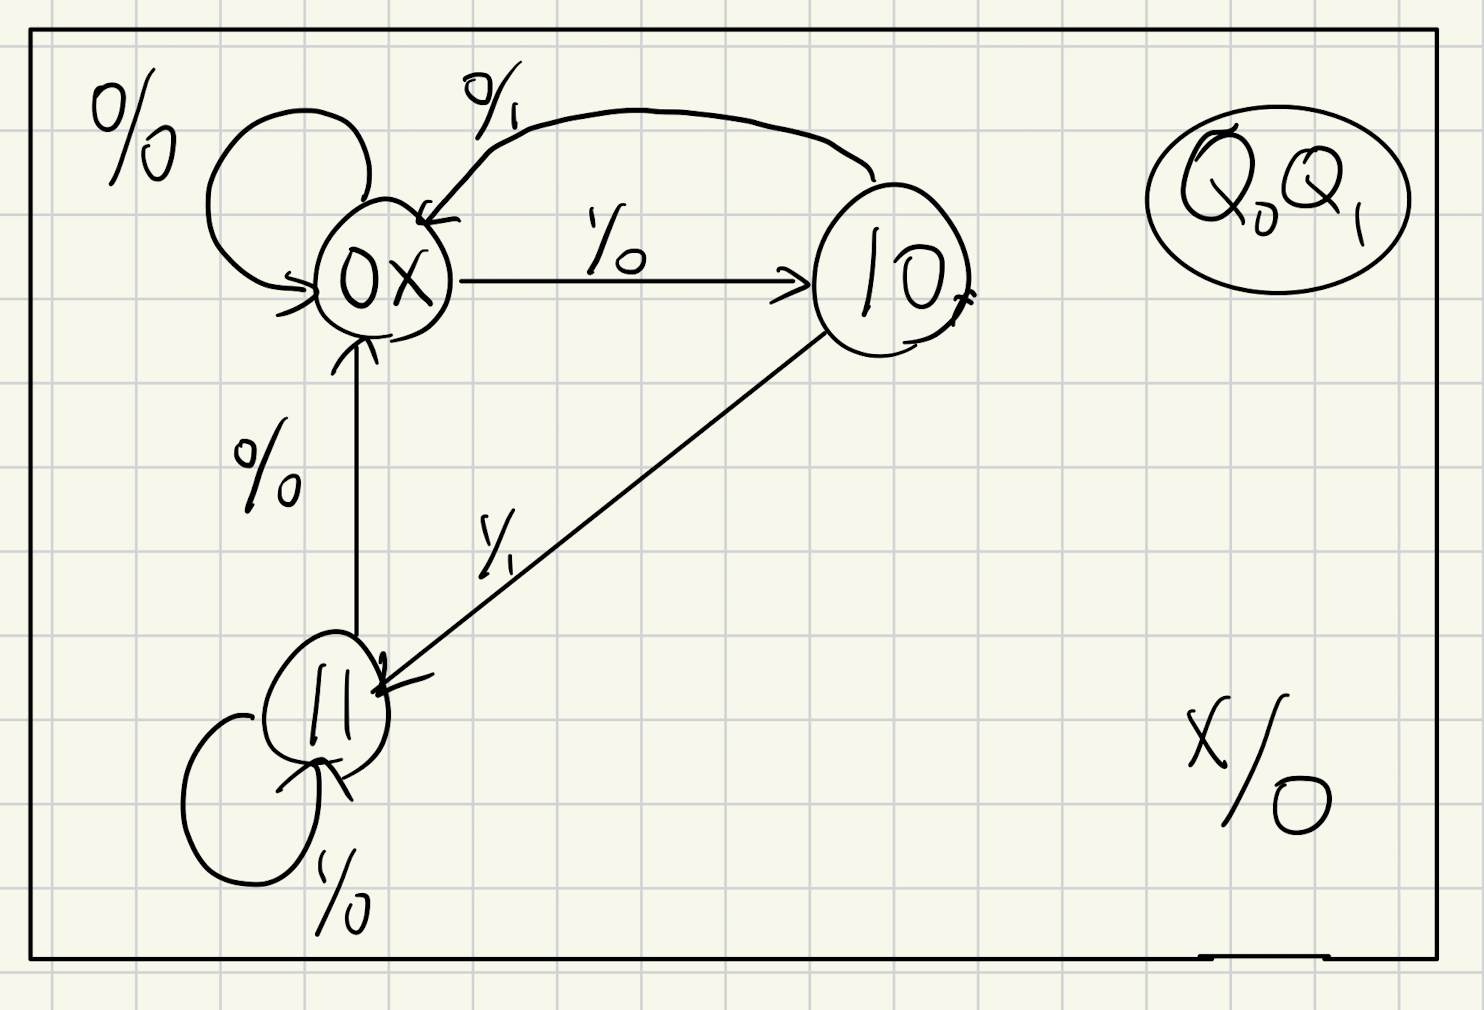
\includegraphics[width=0.8\textwidth]{asset/ex3_state_refine.png}
	\caption{\ref{fig:ex3-state}を簡略化した後の状態遷移図}
	\label{fig:ex3-state-refine}
\end{figure}

\subsection{実際に設計した回路}

\ref{fig:ex3}の回路を,実験資料で示された2ビットカウンタ回路と接続し,
\ref{fig:ex3-cropped}のような回路を設計した.
これをQuartusのRTL Viewerで図持すると\ref{fig:ex3-rtl}のようになる.

\begin{figure}[H]
	\centering
	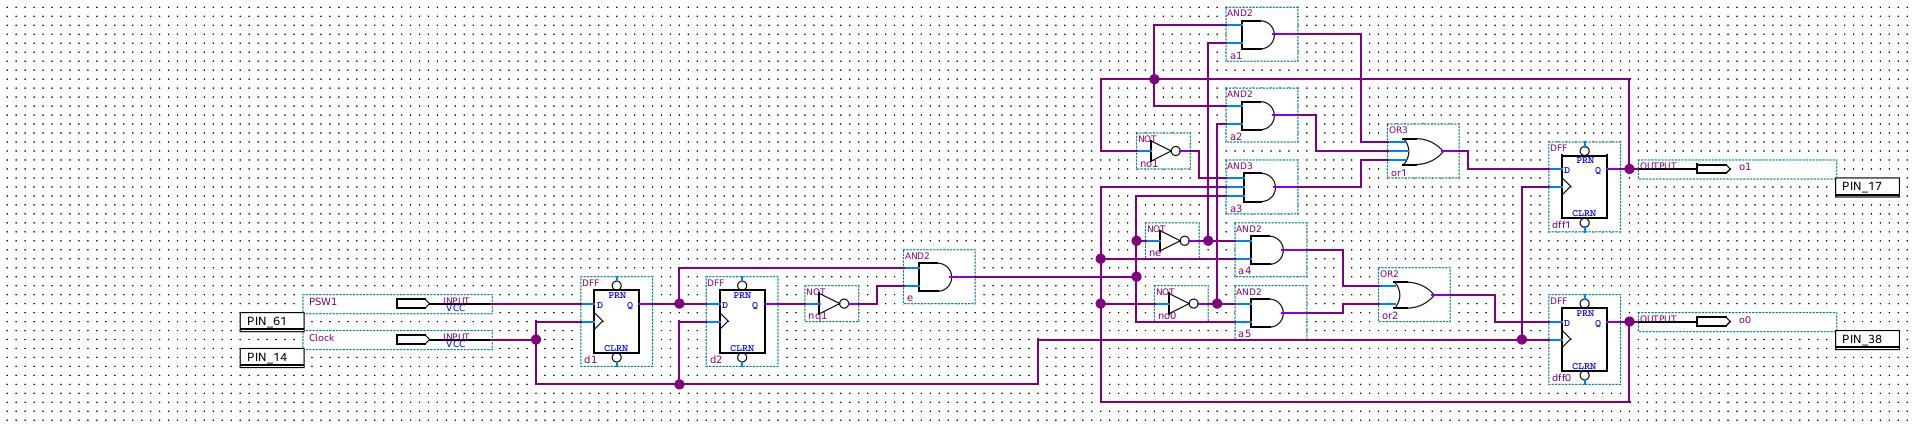
\includegraphics[width=0.8\textwidth]{asset/ex3-cropped.jpg}
	\caption{問題3で設計した回路}
	\label{fig:ex3-cropped}
\end{figure}

\begin{figure}[H]
	\centering
	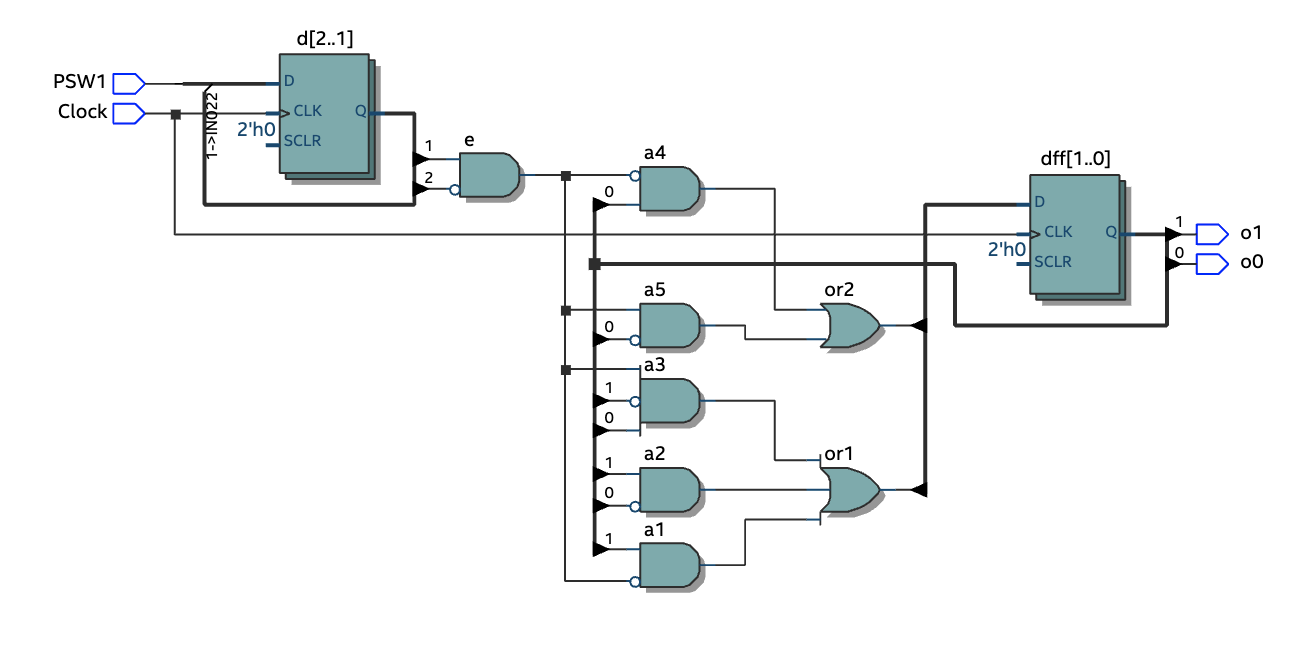
\includegraphics[width=0.8\textwidth]{asset/ex3_pretty.png}
	\caption{\ref{fig:ex3-cropped}をRTL Viewerで表示したもの}
	\label{fig:ex3-rtl}
\end{figure}

\subsection{実験・測定結果}

実際にFPGAボードに書き込み,クロック信号を入力した状態で押しボタンを用いて動作を確認した.
ボタンを押した長さにかかわらず,出力LEDに表示されるカウンタの値が1ずつ増加したので,
微分回路が正常に動作していると考えられる.


\end{document}
